\section{Introducción}

La Discalculia es una discapacidad de aprendizaje específica que afecta la adquisición de habilidades aritméticas. Aunque la falta de  enseñanza, recursos y la baja inteligencia se han relacionado con la etiología de la discalculia, se sabe actualmente que esta discapacidad del aprendizaje es un trastorno cerebral con una predisposición genética familiar \cite{Molko2003}.

\hfill

Por otra parte, hay estudios \cite{Molko2003,Shalev2001} que muestran que una forma de este fenotipo está asociado genéticamente con anomalías tanto funcionales como estructurales del surco intraparietal derecho, llevando esta región un papel fundamental en el desarrollo de las habilidades aritméticas.

\hfill

\begin{center}
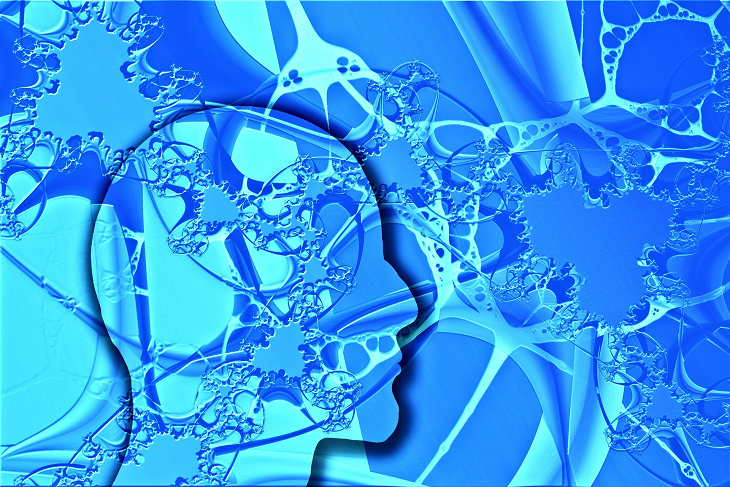
\includegraphics[width=0.79\textwidth]{figures/Neurons.png}
\end{center}

\subsection{Búsqueda del fenotipo}

Para la obtención de más información, hemos utilizado HPO (Human Phenotype Ontology). Este es un vocabulario estandarizado de anomalías fenotípicas en enfermedades humanas que utiliza un fenotipado detallado/preciso para poder ser usado a nivel computacional.

\hfill

Tras realizar una búsqueda del fenotipo a investigar, \textit{Dyscalculia}, vemos que se encuentra clasificado como \href{https://hpo.jax.org/app/browse/term/HP:0002442}{HP:0002442} con un total de 13 fenotipos de otras enfermedades asociadas y un total de 24 genes asociados a esta en HPO.

\hfill

Gracias a las anotaciones en HPO, podemos obtener los genes asociados del fenotipo, y con ello podemos obtener información adicional: Ahora procedemos a la búsqueda de más información a cerca de estos utilizando \href{https://string-db.org}{STRING}, una base de datos biológica y un recurso web de interacciones entre proteínas.

\begin{figure}[b]
	\centering
	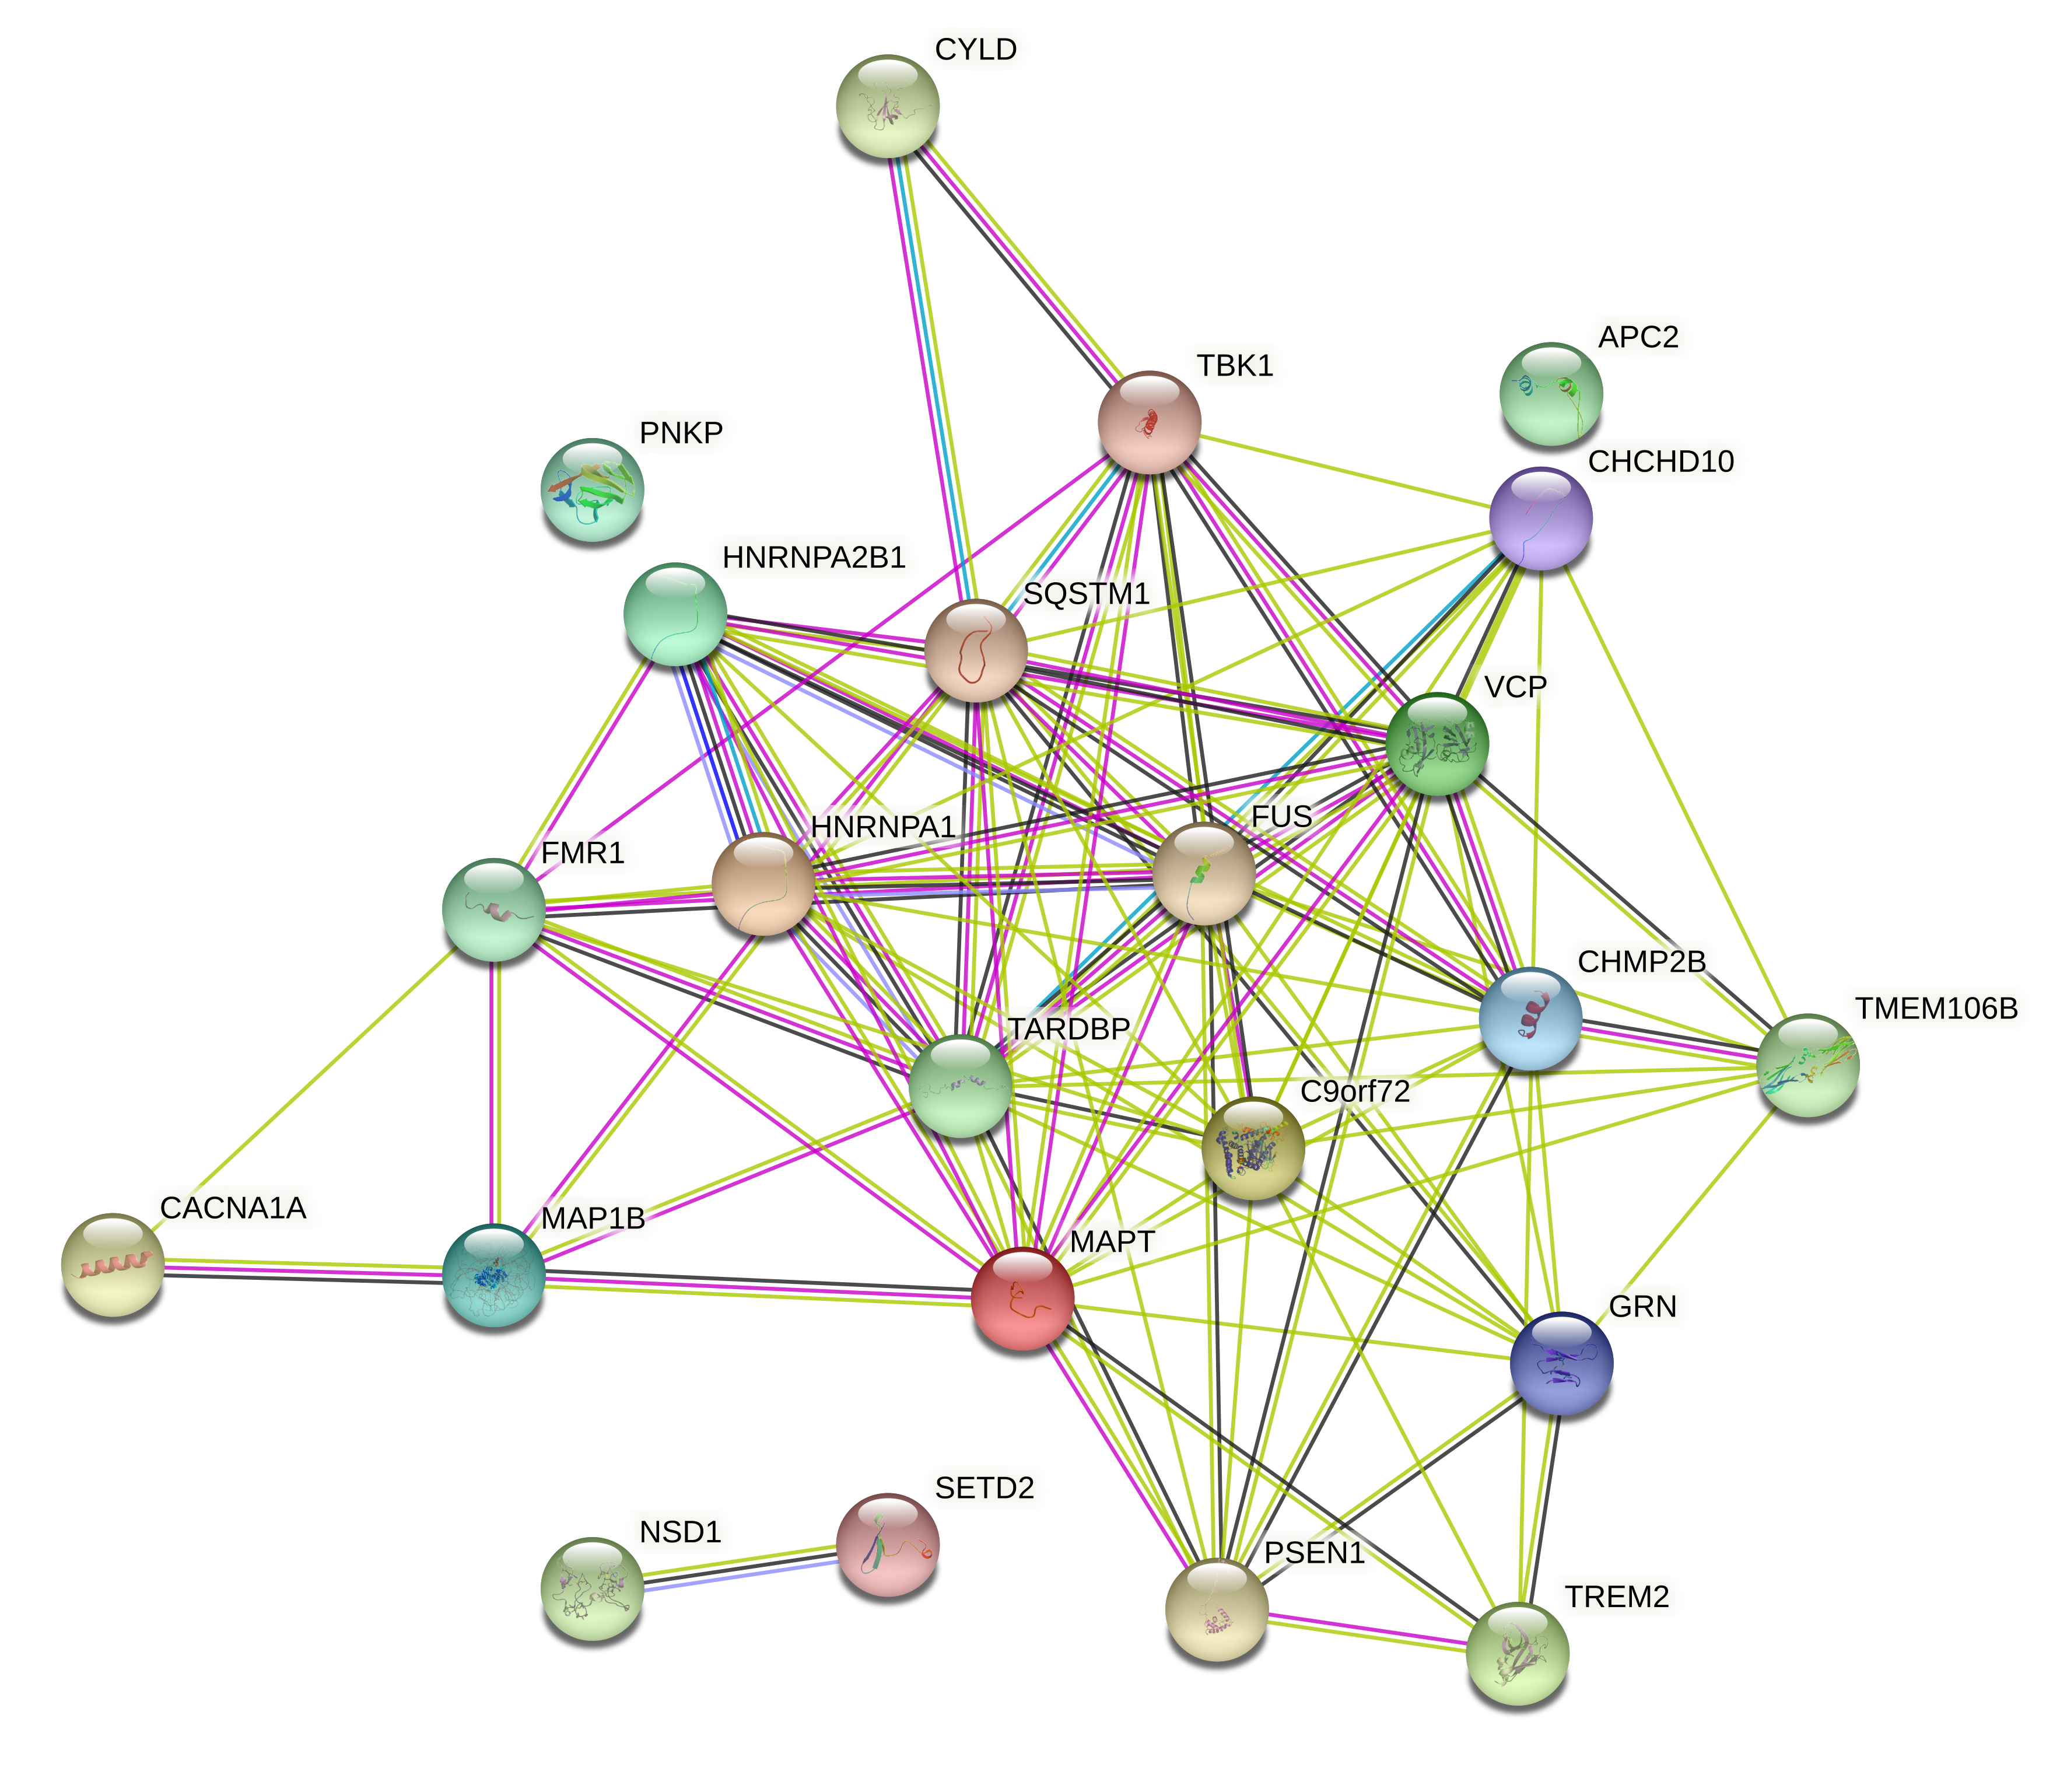
\includegraphics[width=0.50\textwidth]{figures/Gene_Relationship.png}
	\caption{Interacciones proteína-proteína a raíz de los genes relacionados. }
	\label{fig:string1}
\end{figure}


\hfill



\subsection{Búsqueda de interacciones}

Tras investigar las distintas interacciones proteína-proteína (véase la figura \ref{fig:string1}) y observar las enfermedades relacionadas con la discalculia en HPO y los distintos articulos científicos citados anteriormente,suponemos la estrecha relación de la discapacidad con un mal funcionamiento del sistema nervioso. En concreto se podría teorizar que existe una relación con las enfermedades de demencia del complejo frontotemporal del cerebro y la esclerosis lateral amiotrófica, pues estas palabras claves aparecen en la mitad de las enfermedades relacionadas con el fenotipo.

\hfill

Enfermedades como Alzheimer u otras que tienen que ver con demencias fronto-temporales \cite{Walterfang2014} que están también fuertemente relacionadas con un número significativo de proteínas en la red de interacciones mencionada anteriormente.

\hfill

A raíz de los artículos recomendados por la base de datos STRING \cite{Walterfang2014,frontotemporal}, suponemos una relación de estos efectos negativos con una mala conexión entre los hemisferios cerebrales, recordemos que el cerebro delega algunas funciones clave como en este caso puede ser la realización de operaciones matemáticas o el reconocimiento numérico y las interconecta a través del Cuerpo Calloso \cite{CorpusCallosum}. Por tanto, un mal funcionamiento de este elemento del sistema puede llevar a una incapacidad de conexión de las funciones de los distintos hemisferios.

\hfill

\subsection{Información sobre los genes a estudiar}


A continuación se dará una breve información sobre los genes que de mayor grado que hemos encontrado al establecer la red de interconexión del grafo obtenido con String (véase la figura \ref{fig:string1})

\hfill

\textbf{SQSTM1:} Sequestosoma-1; Receptor de autofagia que interactúa directamente tanto con la carga a degradar como con un modificador de autofagia de la familia MAP1 LC3. Puede regular la activación de NFKB1 por TNF-alfa, factor de crecimiento nervioso (NGF) e interleucina-1. Puede desempeñar un papel en la señalización posterior de titina/TTN en las células musculares.\href{https://www.ncbi.nlm.nih.gov/nuccore/NM_001142298.1}{NCBI info}

\hfill

\textbf{FUS:}Proteína de unión a ARN FUS; Se une tanto al ADN monocatenario como al bicatenario y promueve la hibridación independiente de ATP de los ADN monocatenarios complementarios y la formación del bucle D en el ADN superhelicoidal de doble cadena. Puede desempeñar un papel en el mantenimiento de la integridad genómica; Pertenece a la familia RRM TET.\href{https://www.ncbi.nlm.nih.gov/nuccore/NM_001170634.1}{NCBI info}

\hfill

\textbf{VCP:} ATPasa del retículo endoplásmico de transición; Necesario para la fragmentación de las pilas de Golgi durante la mitosis y para su reensamblaje después de la mitosis. Participa en la formación del retículo endoplásmico de transición (tER). La transferencia de membranas desde el retículo endoplásmico al aparato de Golgi se produce a través de vesículas de transición de 50-70 nm que se derivan de elementos de transición parcialmente rugosos y parcialmente lisos del retículo endoplásmico (tER). La formación de vesículas en el tER es un proceso dependiente de ATP. El complejo ternario que contiene UFD1, VCP y NPLOC4 se une a proteínas ubiquitinadas. \href{https://www.ncbi.nlm.nih.gov/nuccore/NM_007126.3}{NCBI info}

\hfill

\textbf{CHMP2B:}Proteína corporal multivesicular cargada 2b; Probable componente central de la clasificación endosomal requerida para el complejo de transporte III (ESCRT-III) que está involucrado en la formación de cuerpos multivesiculares (MVB) y la clasificación de proteínas de carga endosomal en MVB. Los MVB contienen vesículas intraluminales (ILV) que se generan por invaginación y escisión de la membrana limitante del endosoma y, en su mayoría, se envían a los lisosomas, lo que permite la degradación de las proteínas de la membrana, como los receptores del factor de crecimiento estimulado, las enzimas lisosomales y los lípidos.\href{https://www.ncbi.nlm.nih.gov/nuccore/NM_001244644.1}{NCBI info}

\hfill

\textbf{HNRNPA2B1:}Ribonucleoproteínas nucleares heterogéneas A2/B1; Ribonucleoproteína nuclear heterogénea (hnRNP) que se asocia con pre-ARNm nacientes y los empaqueta en partículas de hnRNP. La disposición de las partículas de hnRNP en el hnRNA naciente no es aleatoria y depende de la secuencia, y sirve para condensar y estabilizar las transcripciones y minimizar los enredos y los nudos. El empaque juega un papel en varios procesos, como la transcripción, el procesamiento de pre-ARNm, la exportación nuclear de ARN, la ubicación subcelular, la traducción de ARNm y la estabilidad de los ARNm maduros. Forma partículas hnRNP con al menos otras 20 hnRNP diferentes.\href{https://www.ncbi.nlm.nih.gov/nuccore/NM_002137.3}{NCBI info}